\subsection{Problem Background}
For centuries, people have constructed dams across rivers and streams to hold back water to create reservoirs to manage water supplies. These reservoirs store water for a variety of uses, like agriculture, industry, residential, fishing, preventing downstream flooding, genetating electricity, etc. 
\par
However, with climate changing, the volume of water feeding dams and reservoirs id decreasing in Corolado River.Thus it may not be able to meet the demands for water in Arizona(AZ), California(CA), Wyoming(WY), New Mexico(NM), and Colorado(CO). Moreover, water flow gets lower. This reduces the amount of hydroelectric power generated by the dam. More seriously, if the water level is low enough, hydropower generation will stop.
\begin{figure}[H]
    \centering
    \label{figureIntro}
    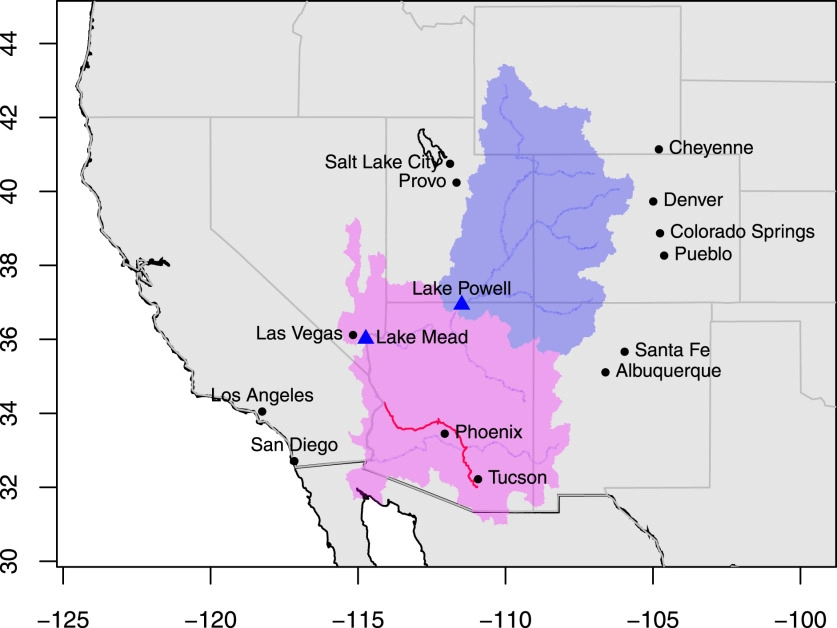
\includegraphics[width=0.9\textwidth]{figures/Map_of_ the_Colorado_River_Basin.png}
    \caption{Map of the Colorado River Basin.}
\end{figure}
\par
The Colorado River Water Allocation Agreement, which was once signed by the states, has allocated more water than the Colorado River currently has. If drought conditions continue in the Colorado River basin, The basic water and power needs of these states will not be met. Consequently,\textbf{We need to find a new water allocation plan}.
\par
According to a recent research~\cite{whitepaper} on Colorado River, the Colorado River has been at or near average for only five of the past 22 years, and below average for the other 17. Hoover Dam's installed capacity is 2,074 megawatts if it is under full storage conditions. Now under drought conditions the capacity is 1,560 megawatts; the storage can provide power to 450,000 households at full capacity, and now it has dropped to about 350,000 households, and its generating capacity has fallen by 25 percent from full capacity.